\section{Auswertung}
\label{sec:Auswertung}

\subsection{Bestimmung der Pulshöhe und Anstiegszeit}
\label{subsec:puls}

In Abbildung \ref{fig:puls} ist beispielhaft ein auf dem Oszilloskop beobachteter Puls
dargestellt. Aus der Abbildung können wie Werte
\begin{align*}
  U_\text{max}&= \SI{11.8}{\volt}\,,\\
  T_\text{Anstieg}&= SI{}{\sec} \text{2/5 von dem was ein Kästchen ist.}
\end{align*}
abgelesen werden.

\begin{figure}
  \centering
  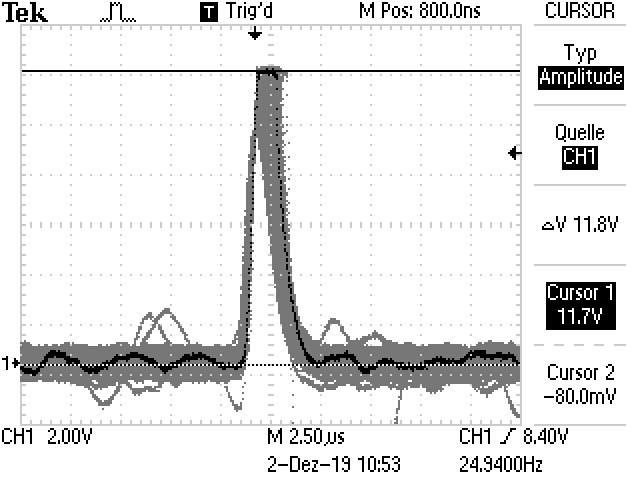
\includegraphics[width=\textwidth]{images/peak.JPG}
  \caption{Darstellung eines Pulses auf dem Oszilloskop.}
  \label{fig:puls}
\end{figure}

\subsection{Bestimmung der Foliendicke}
\label{subsec:dicke}

Die zu Bestimmung der Foliendicke verwendeten Messdaten für die Pulshöhe
mit und ohne Folie befinden sich in Tabelle \ref{tab:dicke}.

\begin{table}[htp]
	\begin{center}
    \caption{Messwerte zur Bestimmung der Foliendicke.}
    \label{tab:dicke}
		\begin{tabular}{cccc}
		\toprule
			{$p_\text{Folie}$/mbar} & {$U_{\text{Folie}}$/V} & {$p$/mbar} & {$U$/V}\\
			\midrule
			107 & 9,84 & 118 & 11,8\\
			114 & 9,52 & 113 & 11,9\\
			126 & 8,96 & 130 & 11,4\\
			140 & 8,24 & 140 & 11,3\\
			148 & 7,20 & 150 & 11,0\\
			156 & 6,88 & 160 & 10,9\\
			163 & 6,32 & 170 & 10,5\\
			177 & 5,84 & 180 & 10,4\\
			187 & 5,20 & 190 & 10,5\\
			199 & 4,08 & 200 & 10,0\\
			- & -  & 213 & 7,9\\
			- & -  & 225 & 8,0\\
			- & -  & 240 & 7,1\\
			- & -  & 250 & 6,0\\
			- & -  & 260 & 4,5\\
			- & -  & 275 & 3,5\\
			- & -  & 285 & 2,6\\
			- & -  & 300 & 2,5\\
		\bottomrule
		\end{tabular}
	\end{center}
\end{table}

Es wird die Pulshöhe in Abhängigkeit vom Druck aufgetragen und für den
linear abfallenden Bereich eine Ausgleichsrechnung der Form
\begin{equation*}
  f(p)=ap+b
\end{equation*}
durchgeführt. Dies ist in Abbildung \ref{fig:dicke} zu sehen. Bei der linearen Ausgleichsrechnung
für die Messreihe ohne Folie werden dabei nur die in blau dargestellten Messwerte berücksichtigt.

\begin{figure}
  \centering
  \includegraphics[width=\textwidth]{build/dicke.pdf}
  \caption{Messwerte für die Messreihen mit und ohne Folie, sowie lineare Ausgleichsrechnungen.}
  \label{fig:dicke}
\end{figure}

Es ergeben sich die Parameter
\begin{align*}
  a_{\text{Folie}}&=\SI{-0.0620(002)}{\volt\per\milli\bar} \, \\
  b_{\text{Folie}}&=\SI{16.61(35)}{\volt} \,\\
  a&=\SI{0.078(005)}{\volt\per\milli\bar} \, \\
  b&=\SI{25.3(11)}{\volt} \,.
\end{align*}

Die Parameter $b$ bzw. $b_{\text{Folie}}$ sind dann die geschätzten Spannungen bei einem vollständig evakuiertem Versuchsaufbau ohne bzw. mit Folie im Strahlengang.
Das Durchlaufen der Folie bedeutet für die Alphateilchen eine Energiedifferenz $\Delta E = E-E_{\text{Folie}}$ bezüglich des Durchlaufens mit bzw. ohne Folie, wobei $E = E_\alpha$ bzw. $E_{\text{Folie}}$ die Energien der Alphateilchen ohne bzw. mit Folie im Weg zum Detektor bezeichnen.
Um nun von Spannungen auf Energien zu schließen, verwendet man den Quotient aus den beiden $y$-Achsenabschnitten, für den
\begin{equation*}
  \frac{b_{\text{Folie}}}{b} = \frac{E_{\text{Folie}}}{E_\alpha}
\end{equation*}
gilt. Mit dieser Information lässt sich die Energiedifferenz durch den Zusammenhang
\begin{equation*}
  \Delta E = E_\alpha \left( 1 - \frac{b_{\text{Folie}}}{b} \right)b_{\text{Folie}}
\end{equation*}
berechnen. Für die vorliegenden Werte ergibt sich $\Delta E = \SI{1.88(18)}{\mega\electronvolt}$.

Die Foliendicke $\Delta s$ wird berechnet, indem die Bethe-Bloch-Formel \eqref{eqn:bethe} als diskreter Energieverlust $\Delta E/(\Delta s \cdot \rho)$ genähert wird.
Dann ergibt sich die Foliendicke durch Umstellen der Formel zu
\begin{equation*}
  \Delta x =
  \frac{m_{\mathrm{e}} v^2(4 \pi \epsilon_{\mathrm{0}})^2}
  {4\pi e^4 z^2 n_\text{Au} \ln{\frac{2 m_{\mathrm{e}} v^2}{I}}}
\end{equation*}.

Die Teilchendichte von Gold lässt sich durch
\begin{equation*}
  N_{\symup{Au}} = N_{\symup{Au}} \frac{\rho_{\symup{Au}}}{M_{\symup{Au}}}
\end{equation*}
berechnen. Mit den Werten $\rho_{\symup{Au}}=\SI{19.32}{\gram\per\cubic\centi\metre}$ \cite{rho}
und ${M_{\symup{Au}}}=\SI{196.97}{\gram\per\mol}$ \cite{molmasse}
ergibt sich der Wert
\begin{equation*}
  N_{\symup{Au}} \approx \SI{5.91e28}{\per\cubic\metre}\,.
\end{equation*}
Die Elektronendichte beträgt dann
\begin{equation}
  N_\text{Au} \cdot Z = N_\text{Au} \cdot 79 \approx \SI{4.66e30}{\per\cubic\metre}\,,
\end{equation}
da jedes Goldatom im Mittel 79 Elektronen enthält, an denen die Alphateilchen streuen können.

Insgesamt beträgt die experimentell bestimmte Foliendicke dann
\begin{equation*}
  \Delta x = \SI{4.4(4)}{\micro\metre}
\end{equation*}
mit einer relativen Unsicherheit von $9{,}09\%$.

\subsection{Bestimmung des Raumwinkels}
\label{subsec:raumwinkel}

Der Raumwinkel $\Delta \Omega$ ist der Raumwinkel um die Folie herum, der die
effektive Detektorfläche beschreibt. Die effektive Detektorfläche folgt aus geometrischen
Überlegungen. Diese sind in Abbildung \ref{fig:skizze} veranschaulicht.

\begin{figure}
  \centering
  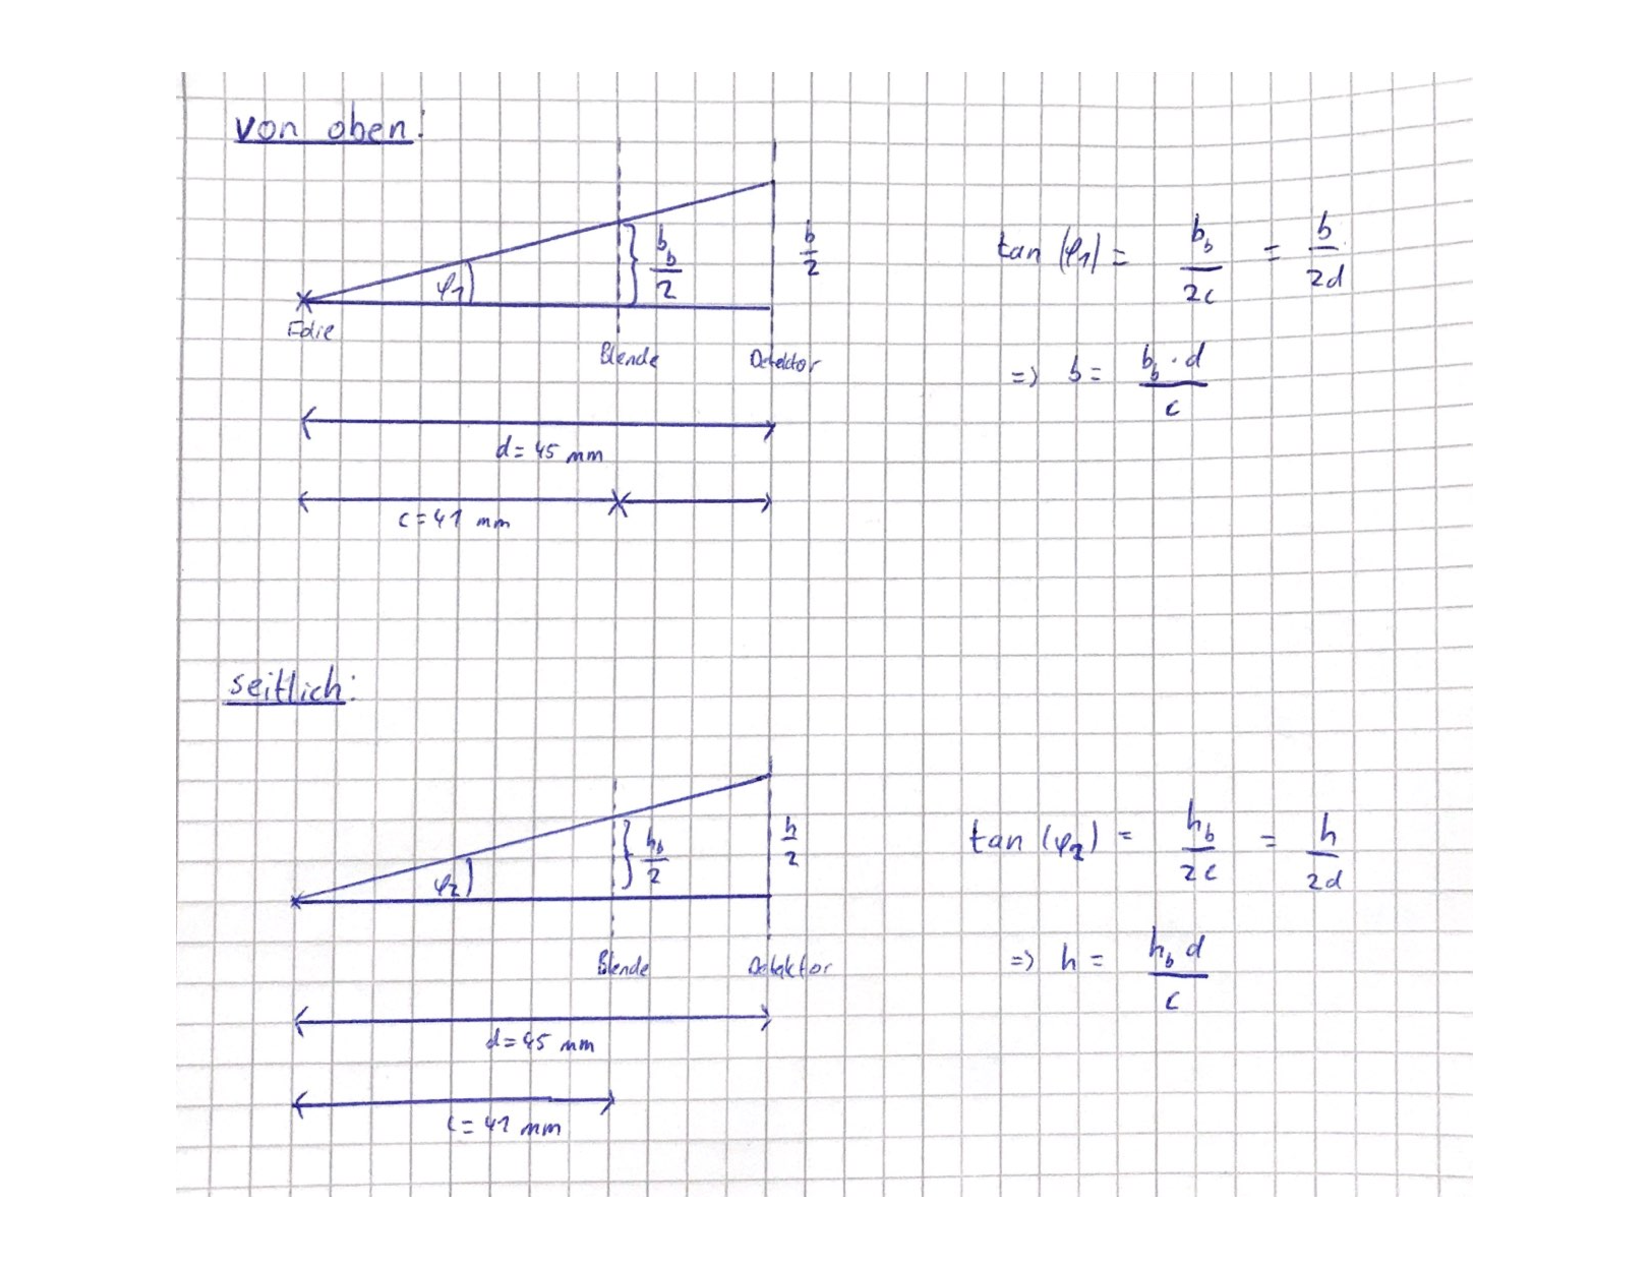
\includegraphics[width=\textwidth]{images/skizze.pdf}
  \caption{Skizze zur Berechnung der Größen $b$ und $h$ aus der Geometrie des Versuchsaufbaus.}
  \label{fig:skizze}
\end{figure}

Aus trigonometrischen Verhältnissen kann hergeleitet werden, dass gilt:
\begin{align*}
  b &= \frac{b_{\symup{b}} d}{c} \,,\\
  h &= \frac{h_{\symup{b}} d}{c} \,.
\end{align*}
Dabei bezeichnet $b_{\symup{b}}$ die Breite und $h_{\symup{b}}$ die Höhe der Blende.
Die Breite der effektiven Detektorfläche wird mit $b$ bezeichnet und die entsprechende Höhe mit $h$.
Der Abstand von der Folie zur Blende ist durch $c$ gegeben und $d$ beschreibt den Abstand
der Folie und der Detektoroberfläche. Aus den bekannten Werten \cite{Versuchsanleitung}
\begin{align*}
  b_{\symup{b}} &= \SI{2}{\milli\meter} \,, \\
  h_{\symup{b}} &= \SI{10}{\milli\meter} \,, \\
  c &= \SI{41}{\milli\meter} \,,\\
  d &= \SI{41}{\milli\meter}
\end{align*}
lassen sich die Werte
\begin{align*}
  b &= \SI{2.195}{\milli\meter} \,,\\
  h &= \SI{10.976}{\milli\meter}
\end{align*}
berechnen. Diese charakterisieren die effektive Detektorfläche. Der Raumwinkel kann dann durch
\begin{equation}
  \Delta \Omega = 4 \arctan\left(\frac{b h}{2d \sqrt{4d^2 + b^2 + h^2}}\right)
\end{equation}
berechnet werden \cite{raumwinkel}. Mit den oben genannten Werten ergibt sich
\begin{equation*}
  \Delta \Omega = \SI{0.0118}{sr} \,.
\end{equation*}

Der Raumwinkel um die Quelle herum folgt mit den Werten \cite{Versuchsanleitung}
\begin{align*}
  c &= \SI{97}{\milli\meter} \,, \\
  d &= \SI{101}{\milli\meter}
\end{align*}
zu
\begin{equation*}
  \Delta \Omega_\text{Quelle} = \SI{0.0021}{sr} \,.
\end{equation*}

(WELCHEN RAUMWINKEL MÜSSEN WIR JETZT NEHMEN? DER DER QUELLE ERSCHEINT MIR SINNVOLLER...)

\subsection{Bestimmung der Aktivität der Probe}
\label{subsec:aktivitaet}

Die theoretisch heute zu erwartende Aktivität lässt sich mit Kenntnis der Halbwertszeit
und der Aktivität zu einem früheren Zeitpunkt berechnen. Im Oktober 1994 betrug die
Aktivität der Probe $\SI{330}{\kilo\becquerel}$ \cite{Versuchsanleitung}. Die Halbwertszeit
von 241-Americium beträgt $T_{1/2}=432$ Jahre. Daraus lässt sich mithilfe von
\begin{align*}
  A_{\text{heute,theo}}&= A_{1994}\exp(-\lambda t) \, \\
  \lambda&= \frac{\ln(2)}{T_{1/2}}
\end{align*}
die heutige Aktivität bestimmen. Die Zeit beträgt dabei $t=25+1/6$ Jahre. Somit beträgt die
theoretisch zuerwartende heutige Aktivität
\begin{equation*}
  A_{\text{heute,theo}}= \SI{316.94}{\kilo\becquerel} \,.
\end{equation*}

Aus den Messwerten lässt sich die heutige Aktivität unter
Kenntnis des Raumwinkels $\Delta \Omega_{\text{Quelle}}$ aus der Messung der Zählrate berechnen.
Das Verhältnis der heutigen Aktivität und die gemessene Zählrate müssen nämlich in
dem gleichen Verhältnis zueinander stehen, wie der Raumwinkel $\Delta \Omega_{\text{Quelle}}$ und
der gesamte Raumwinkel. Somit ist die heutige Aktivität gegeben durch
\begin{equation*}
  A_{\text{heute,exp}}=\frac{4 \pi  I}{\Delta \Omega_{\text{Quelle}}}=\SI{}{\kilo\becquerel} \,.
\end{equation*}


\subsection{Bestimmung des differentiellen Wirkungsquerschnitts}
\label{subsec:wq}


In Tabelle \ref{tab:wq} sind die Messwerte für die Zählrate in Abhängigkeit vom
Winkel aufgeführt. Die Zählzeiten wurden dabei manuell mithilfe einer Stoppuhr bestimmt.
Außerdem befinden sich dort die berechneten differentiellen
Wirkungsquerschnitte. Das Vorgehen zur Berechnung der Wirkungsquerschnitte wird im
Folgenden erläutert.
\begin{table}[htp]
	\begin{center}
    \caption{Messwerte zur Bestimmung des differentiellen Wirkungsquerschnitts, sowie
    die daraus berechneten Aktivitäten und Wirkungsquerschnitte.}
    \label{tab:wq}
		\begin{tabular}{ccccc}
		\toprule
			{$N$} & {$t$/s} & {$I/\mathrm{s^-1}$} & {$\theta$/°} & ${\frac{d\sigma}{d \Omega}}$\\
			\midrule
			1214 \pm 35 & 150  & 8,09 \pm 0,23 &  0,00 & 1,85 \pm 0,07\\
			1271 \pm 36 & 170  & 7,48 \pm 0,21 & -0,50 & 1,71 \pm 0,06\\
			1185 \pm 34 & 180  & 6,58 \pm 0,19 & -1,00 & 1,50 \pm 0,05\\
			1072 \pm 33 & 180  & 5,96 \pm 0,18 & -1,50 & 1,36 \pm 0,05\\
			1109 \pm 33 & 200  & 5,54 \pm 0,17 & -2,00 & 1,27 \pm 0,05\\
			1103 \pm 33 & 200  & 5,51 \pm 0,17 & -2,50 & 1,26 \pm 0,05\\
			930  \pm 31 & 210  & 4,43 \pm 0,15 & -3,00 & 1,01 \pm 0,04\\
			783  \pm 28 & 210  & 3,73 \pm 0,13 & -3,50 & 0,85 \pm 0,04\\
			881  \pm 30 & 210  & 4,20 \pm 0,14 & -4,00 & 0,96 \pm 0,04\\
			854  \pm 29 & 210  & 4,07 \pm 0,14 & -4,50 & 0,93 \pm 0,04\\
			522  \pm 23 & 210  & 2,49 \pm 0,11 & -5,00 & 0,57 \pm 0,03\\
			540  \pm 23 & 270  & 2,00 \pm 0,09 & -5,50 & 0,46 \pm 0,02\\
			533  \pm 23 & 270  & 1,97 \pm 0,09 & -6,00 & 0,45 \pm 0,02\\
			1156 \pm 34 & 150  & 7,71 \pm 0,23  & 0,50 & 1,76 \pm 0,06\\
			1461 \pm 38 & 170  & 8,59 \pm 0,22  & 1,00 & 1,96 \pm 0,07\\
			1269 \pm 36 & 150  & 8,46 \pm 0,24  & 1,50 & 1,93 \pm 0,07\\
			1248 \pm 35 & 150  & 8,32 \pm 0,24  & 2,00 & 1,90 \pm 0,07\\
			1229 \pm 35 & 150  & 8,19 \pm 0,23  & 2,50 & 1,87 \pm 0,07\\
			1328 \pm 36 & 150  & 8,85 \pm 0,24  & 3,00 & 2,02 \pm 0,07\\
			1258 \pm 35 & 150  & 8,39 \pm 0,24  & 3,50 & 1,91 \pm 0,07\\
			1428 \pm 38 & 150  & 9,52 \pm 0,25  & 4,00 & 2,17 \pm 0,07\\
			1251 \pm 35 & 150  & 8,34 \pm 0,24  & 4,50 & 1,90 \pm 0,07\\
			1160 \pm 34 & 150  & 7,73 \pm 0,23  & 5,00 & 1,77 \pm 0,06\\
			1165 \pm 34 & 150  & 7,77 \pm 0,23  & 5,50 & 1,77 \pm 0,06\\
			933  \pm 31 & 150  & 6,22 \pm 0,20  & 6,00 & 1,42 \pm 0,05\\
			811  \pm 28 & 150  & 5,41 \pm 0,19  & 6,50 & 1,23 \pm 0,05\\
			941  \pm 31 & 180  & 5,23 \pm 0,17  & 7,00 & 1,19 \pm 0,05\\
			756  \pm 28 & 180  & 4,20 \pm 0,15  & 7,50 & 0,96 \pm 0,04\\
			762  \pm 28 & 210  & 3,63 \pm 0,13  & 8,00 & 0,83 \pm 0,03\\
			622  \pm 25 & 210  & 2,96 \pm 0,12  & 8,50 & 0,68 \pm 0,03\\
			511  \pm 23 & 210  & 2,43 \pm 0,11  & 9,00 & 0,56 \pm 0,03\\
			502  \pm 22 & 240  & 2,09 \pm 0,09  & 9,50 & 0,48 \pm 0,02\\
			409  \pm 20 & 240  & 1,70 \pm 0,08  & 10,00& 0,39 \pm 0,02\\
		\bottomrule
		\end{tabular}
	\end{center}
\end{table}

Für den Wirkungsquerschnitt gilt \cite{wq}:
\begin{equation}
  \frac{\symup{d}\sigma}{\symup{d}\Omega} = \frac{I}{I_0  N_{\symup{Au}} \Delta x \Delta \Omega} \,.
  \label{eqn:wq}
\end{equation}
Dabei ist $I$ die Zählrate mit Folie, $I_0$ die Zählrate ohne Folie, $ N_{\symup{Au}} \approx \SI{5.91e28}{\per\cubic\metre}$
die Teilchendichte von Gold, $\Delta x$ die Foliendicke und $\Delta \Omega$ der Raumwinkel.
Mit der Zählrate $I_0=\SI{15.73(032)}{1 \per\second}$ ohne Folie, der Schichtdicke $\Delta x =2$\,µm und dem Raumwinkel
aus Kapitel \ref{subsec:raumwinkel} ergeben sich damit die in Tabelle \ref{tab:wq} dargestellten Werte.

Diese sind in Abbildung \ref{fig:wq} gegen den Streuwinkel $\theta$ aufgetragen. Außerdem ist
eine Theoriekurve zu sehen. Diese wird gemäß Gleichung \eqref{eqn:rutherford} mit den
Werten $z=2$, $Z=79$ und $E=5{,}5$\,MeV \cite{energie} berechnet.

\begin{figure}
  \centering
  \includegraphics[width=\textwidth]{build/wq.pdf}
  \caption{Berechnete Werte für den differentiellen Wirkungsquerschnitt und Theoriekurve.}
  \label{fig:wq}
\end{figure}

Die Fehler werden hier nach der Gauß'schen Fehlerfortpflanzung bestimmt:
\begin{equation*}
  \sigma_{\frac{\symup{d}\sigma}{\symup{d}\Omega}} = \sqrt{\left(\frac{\sigma_N}{t \cdot I_0 \cdot N_{\symup{Au}} \cdot \Delta x \cdot \Delta \Omega}\right)^2
  + \left(\frac{N \cdot \sigma_{I_0}}{t \cdot I_0^2 \cdot N_{\symup{Au}} \cdot \Delta x \cdot \Delta \Omega}\right)^2}
\end{equation*}


\subsection{Untersuchung von Mehrfachstreuung}
\label{subsec:mehrfach}

Für zwei Goldfolien mit den Dicken $\Delta x=2$\,µm und $\Delta x=4$\,µm werden
die Zählraten
\begin{align*}
  I_2&= \SI{15.71(32)}{1\per\second}\,,\\
  I_4&= \SI{17.18(34)}{1\per\second}
\end{align*}
gemessen. Analog zu der Berechnung in Kapitel \ref{subsec:wq} lassen sich die Wirkungsquerschnitte
\begin{align*}
  \left(\frac{d \sigma}{d \Omega}\right)_2&=\SI{3.92(11)e-21}{\metre\squared} \,, \\
  \left(\frac{d \sigma}{d \Omega}\right)_4&=\SI{1.79(05)e-21}{\metre\squared}
\end{align*}
berechnen. Es ist erkennbar, dass der Wirkungsquerschnitt für die dünnere Folie
größer ist.

Da der Winkel bei dieser Messung zu $\theta=0°$ gewählt wurde und die
Rutherford'sche Streuformel \eqref{eqn:rutherford} an dieser Stelle eine Polstellt beseitzt,
können die theoretischen Werte hier nicht berechnet werden.

\subsection{Untersuchung der $Z$-Abhängigkeit}
\label{subsec:z}

Zur Untersuchung der Mehrfachstreuung wurden Folien aus Gold, Platin und
Bismut untersucht. In Tabelle \ref{tab:elemente} sind die Dicken $\Delta x$ der Folien,
die Ordnungszahlen $Z$ \cite{molmasse}, die Dichten $\rho$ \cite{rho}, die molaren Massen $M$
\cite{molmasse} und die daraus berechneten
Parameter $\frac{I}{N \Delta x}$ aufgeführt. $N$ bezeichnet hier die in Kapitel \ref{subsec:wq}
bereits eingeführte Teilchendichte des jeweiligen Elements.

\begin{table}[htp]
	\begin{center}
    \caption{Messdaten, sowie Daten der Elemente und daraus berechnete Werte.}
    \label{tab:elemente}
		\begin{tabular}{cccccccc}
		\toprule
    {Element}&{$N$}  & {$I/\mathrm{s^{-1}}$} & {$\rho/\frac{\mathrm{g}}{\mathrm{cm}^3}$}
    & {$M/\frac{\mathrm{g}}{\mathrm{Mol}}$} & {$x$/µm} & {$Z$} & {$\frac{I}{Nx}/\frac{\mathrm{m}^2}{\mathrm{s}}$}\\
			\midrule
      Au  &  905 \pm 30 & 1,89 \pm 0,06 & 19,32 & 196,97 & 2 & 79 & 1,60\\
      Au  &  836 \pm 29 & 1,74 \pm 0,06 &  19,32 & 196,97 & 4 & 79 & 0,74\\
      Pt  &  901 \pm 30 & 1,88 \pm 0,06 &  21,45 & 195,09 & 2 & 78 & 1,42\\
      Bi  &  985 \pm 31 & 2,05 \pm 0,07 &   9,80 & 208,98 & 1 & 83 & 7,27\\
		\bottomrule
		\end{tabular}
	\end{center}
\end{table}

In Abbildung \ref{fig:z} ist der Parameter $\frac{I}{N \Delta x}$ gegen die Ordnungszahl
aufgetragen. Es sind dabei zwei Werte bei $Z=79$ zu sehen, da zwei unterschiedlich dicke
Goldfolien untersucht wurden. Es ist zu erkennen, dass der Parameter $\frac{I}{N \Delta x}$
tendenziell mit der Ordnungszahl zunimmt.

\begin{figure}
  \centering
  \includegraphics[width=\textwidth]{build/z.pdf}
  \caption{Auftragung des Parameters $\frac{I}{N \Delta x}$ gegen die Ordnungszahl $Z$.}
  \label{fig:z}
\end{figure}

(IN DER ANLEITUNG STEHT MAN SOLL DAS JETZT NOCH IRGENDWIE THEORETISCH BERECHNEN...)
Dafür einfach Rutherford durch einen Wert teilen für den gegebenen Winkel. Dann kann
man das auch gegen Z auftragen.
